%%%%%%%%%%%%%%%%%%%%%%%%%%%%%%%%%%%%%%%%%%%%%%%%%%%%%%%%%%%%%%%%%
%2345678901234567890123456789012345678901234567890123456789012345
%        1         2         3         4         5         6     
\chapter{Experimental result}
\label{cha:experiment}
 The experiment is conducted both in simulation and ABB test prototype through collecting sensor feedback and apply forward kinematic on it.
The main design objective of our controller is it's performance under inconsistent task space command. 

In this chapter we test 3 trajectories each represent a typical situation. 
\begin{itemize}
    \item[1] Pure rotation trajectory. From initial position, the platform makes a 360 degree rotation while the $\dot{x},\dot{y}$ remains 0 all the time.
    \item[2] 90 degree turn of heading. The task space velocity change from $\dot{\xi}=[1,0,0]$ to $\dot{\xi}=[0,1,0]$ in one control cycle.
    \item[3] Translation with rotation. Move 10 meters along x direction and rotate 360 degree simultaneously
\end{itemize}
The pure rotation trajectory require a sudden change of ICR position from infinite far away to origin, which corresponding to a 45 degree sudden change on steering angles. This most part of this trajectory will trigger the ICR control logic so it is used to test the ICR controller performance.

The 90 degree turn trajectory does not involve and angular velocity so the ICR is always infinite far away, thus only approximation based inverse kinematic control logic will be triggered. Thus this trajectory is used to test the performance of IKAM control logic.

The translation with rotation trajectory represents the general cases, where the task space command is generally smooth and ICR is changing position so that switching between 2 control logics happens frequently. Thus this trajectory is to test the general performance and the switching.
\begin{table}[b]
	\centering
		\begin{tabular}{cc}
		Trajectories   &  control strategy triggered                  \\\midrule
		Pure rotation          &  ICR, IKAM     \\
		90 degree turn          &  IKAM              \\
		Translation with rotation      &  ICR, IKAM              \\\bottomrule
		\end{tabular}
		\vspace{1mm}
	\caption{Nomenclature of the MPC approaches}
	\label{tab:testTrajectory}
\end{table}
This chapter is then divided by 4 sections, 3 of them explain 3 test trajectory and the last section discuss the advantage and problem we observe in the experiment.

\section{Preliminaries}
\label{sec:setup}

For the optimal growth of tomato crop an air temperature of \unit{25}{°C} and an relative air humidity of \unit{65}{\%} are assumed.
That equals at the given temperature an absolute air humidity of \unit{0.015}{g} water per cubic metre of air.
The quadratic objective function used was:
\begin{equation}\label{eq:objective_setpoint}
J_{sp} = 200 \cdot (25.0 - X_{T,a})^2 + 100 \cdot (0.015 - X_{H_{a,a}})^2,
\end{equation}
which enforces temperature tracking more than humidity tracking of the previously mentioned optimal conditions.

The full description of the set-point tracking MPC is given by:
\begin{subequations}\label{eq:setup_setpoint}
\begin{align}
\min \, \int_{0}^{t_f} \! J_{sp} \, \mathrm{d}t
\end{align}
subject to:
\begin{align}
\dot{\mathbf{x}}_{pm}(t) = f(\mathbf{x}(t),\mathbf{u}(t);\mathbf{d}(t)),\\
\mathbf{u}(t) \in \mathcal{U}, 
\end{align}
\end{subequations}
where $\dot{\mathbf{x}}_{pm}$ is the model equation of the corresponding MPC approach.
Since set-point tracking shows the ability to keep a system close to the desired state no state constraints were defined is it can be seen in \cref{tab:varconstraints_setpoint}.

\begin{table}[htb]
	\centering
		\begin{tabular}{cccc}
		quantities                    &  lower bound     &  upper bound     &  unit                  \\\midrule
$X_{T,a}$        &  -     & -     &  $\unit[]{^\circ C}$   \\
$X_{H_{a,a}}$    &  -   &  -   &  $\unit[]{kg/m^3}$     \\
$U_{ven}$        &  \unit[1]{}    &  \unit[100]{}    &  $\unit[]{\%}$         \\
$U_{shd}$        &  \unit[0]{}      &  \unit[0.7]{}    &  $\unit[]{-}$          \\
$U_{heat}$       &  \unit[0]{}      &  \unit[1000000]{}&  $\unit[]{W/m^2}$      \\
$U_{hum}$        &  \unit[0]{}      &  \unit[0.2]{}    &  $\unit[]{\nicefrac{kg}{m^5 \cdot s}}$   \\\bottomrule
\end{tabular}
\vspace{1mm}
	\caption{Constraints of the controlled variables $X_{(\cdot)}$ and manipulated variables $U_{(\cdot)}$.}
	\label{tab:varconstraints_setpoint}
\end{table}

\section{Pretests}
\label{sec:pretests}

A deep analysis of LMPC+GP was done on noise-free predictions in \cref{sec:noisefree} because noise-free predictions enable explicitly to quantify the profit of the LMPC+GP scheme.
In this section the three aspects disturbance prediction, error estimation with linear kernels and performance with noisy disturbances are emphasized.

Stressing MPC considering the weather forecast is motivated by being able to reject the effect of disturbance variables.
This is illustrated in \cref{fig:benefit_mpc}.
The settings of the both pictured NMPC approaches differ only in the prediction of the disturbance variables.
Including variable and exact predictions in the computations enables the control to reject disturbances in advance and to stick very close to the set-point.
Whereas assuming constant disturbance values over the prediction horizon leads to major deviations since the control has to react to the current disturbances.

\begin{figure}[!t]
\begin{center}
		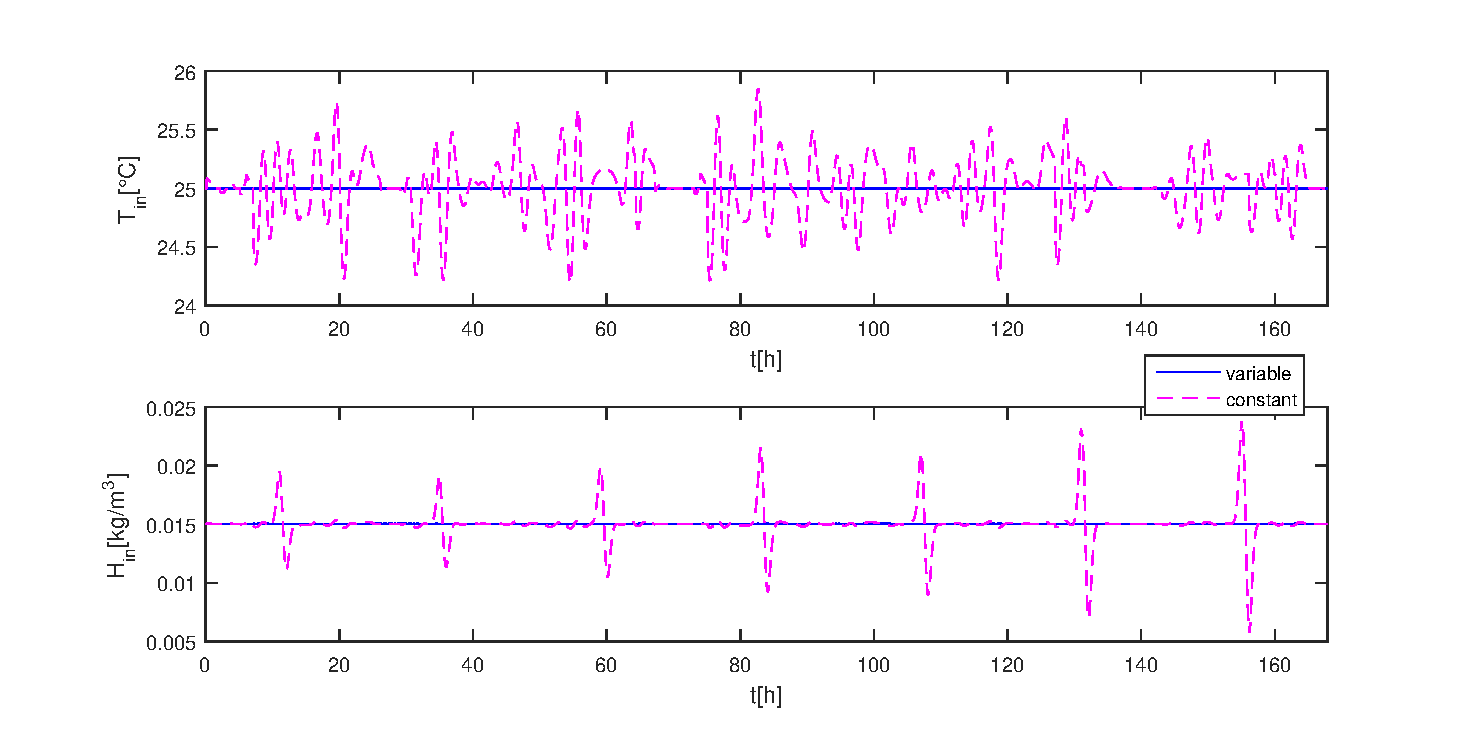
\includegraphics[width=\textwidth]{../Figures/benefit_mpc.eps}
		\caption{Comparison of NMPC with variable and constant disturbance prediction}
		\label{fig:benefit_mpc}
\end{center}
\end{figure}

Due to the fact that GPs with linear kernels can be directly included into the optimization of a linear MPC scheme, this setup denoted as LMPC+LGP was tested.
But the linear kernels were not able to model the error as \cref{fig:mpc_linear_kernels} depicts.
When the input variables for the GP were in a scope where the linear kernels modelled the error well, the control quality of LMPC+GP was similar to LMPC (e.g. at $t \approx \unit{100}{h}$).
But for extrapolating outside their scope the linear kernels led to massive deviations from the set-point (e.g. at $t \approx \unit{65}{h}$).
Since the error is the by the linearisation neglected nonlinear dynamics it inherits the nonlinear characteristics.
Thus, nonlinear approach is required to model the error properly.
Hence, the approach with linear kernels was dropped.

\begin{figure}[!t]
\begin{center}
		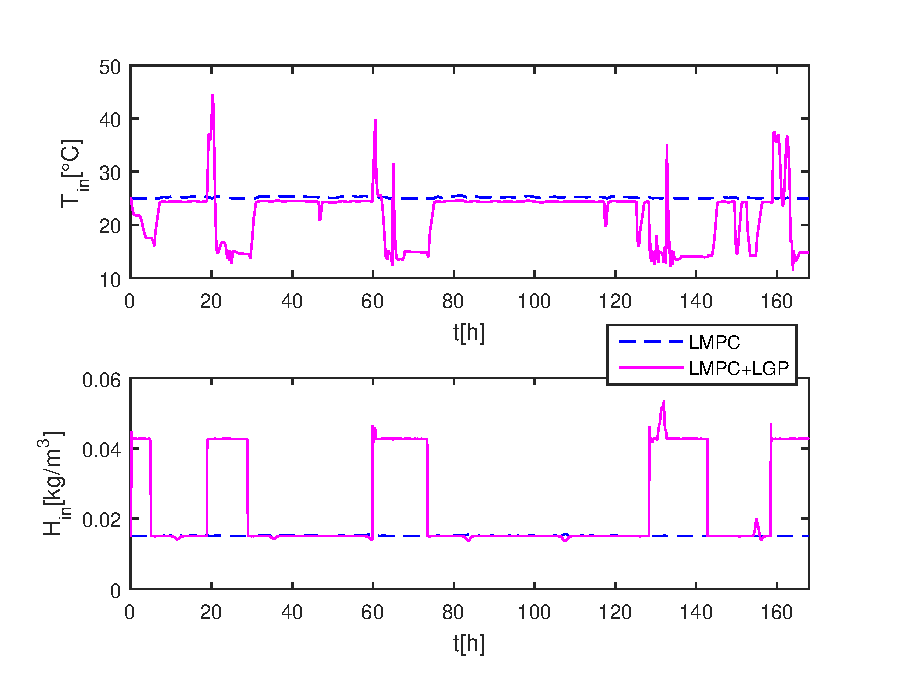
\includegraphics[width=\textwidth]{../Figures/linear_kernel.eps}
		\caption{Comparison of augmented MPC with solely linear kernels and linear MPC}
		\label{fig:mpc_linear_kernels}
\end{center}
\end{figure}

Since signals from sensors are noisy and the weather forecast is non perfect the application of MPC in a real greenhouse has to handle the outcomes.
Thus, the ability of LMPC+GP to cope with noisy predictions was checked to simulate a more realistic scenario.
\cref{fig:noisy_mpc} depicts the results for NMPC and LMPC+GP in which NMPC serves as the benchmark.
Due to the non perfect predictions MPC is not able to compute the optimal input.
Therefore, the state trajectories are chattering around the set-points.
Since both approaches are able to track the set-points and the results of NMPC and LMPC+GP are matchable it is shown that LMPC+GP is able to handle noisy predictions.

\begin{figure}[!t]
\begin{center}
		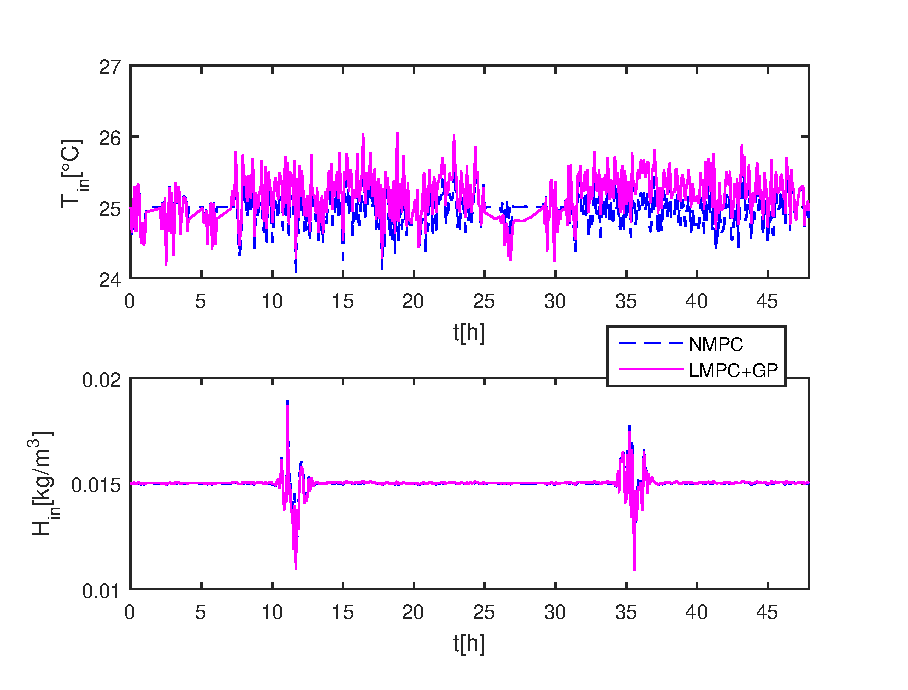
\includegraphics[width=\textwidth]{../Figures/setpoint_noise.eps}
		\caption{Comparison of nonlinear and augmented MPC with noisy predictions}
		\label{fig:noisy_mpc}
\end{center}
\end{figure}

\section{Noise-free tracking}
\label{sec:noisefree}

The comparison of NMPC, LMPC and LMPC+GP was done on noise-free predictions.
Thus, the benefit of LMPC+GP can be clearly ascertained eliminating the random effect of noise.
For all three schemes the prediction horizon was eight hours and the sample period was fixed to five minutes.
The aim of achieving a performance with a linear MPC scheme similar to a NMPC scheme was reached.

The progress of the state trajectories is depicted in \cref{fig:setpoint_states}.
NMPC is the benchmark for LMPC and LMPC+GP as it uses the nonlinear prediction model which is identical to the simulation model portrayed in \cref{cha:ICR}.
Therefore, the results are optimal with respect to the objective function \eqref{eq:objective_setpoint}.

\begin{figure}[!t]
\begin{center}
	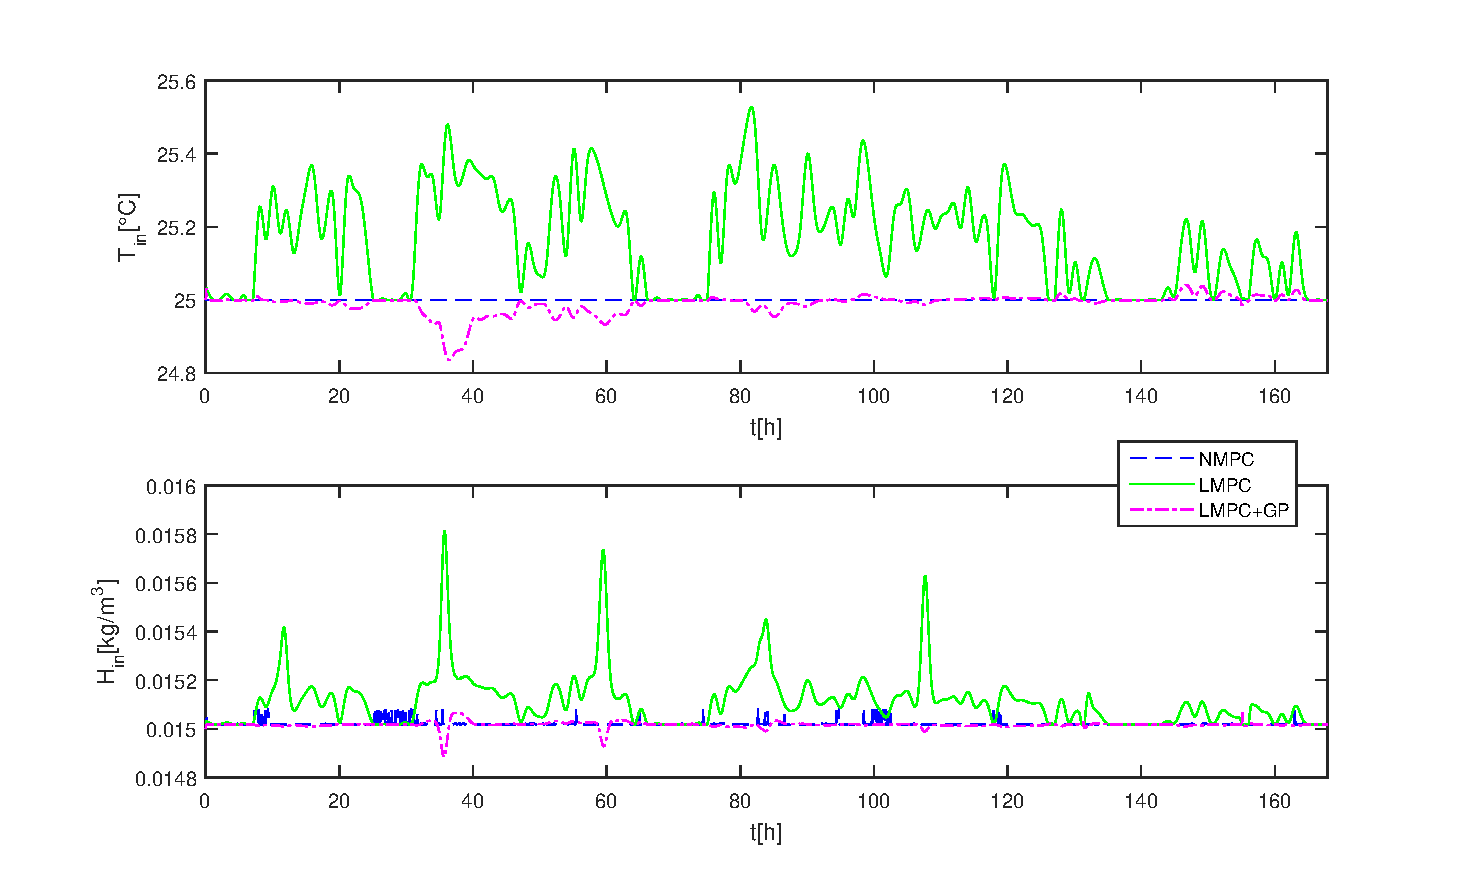
\includegraphics[width=\textwidth]{../Figures/setpoint_states.eps}
	\caption{State trajectories}
	\label{fig:setpoint_states}
\end{center}
\end{figure}

LMPC and LMPC+GP use the same prediction model except for the error term added in LMPC+GP.
By estimating the error with GPs LMPC+GP achieves a diminishing of the square root tracking error by more than \unit[86]{\%} for both temperature and humidity.
Also the  maximum deviation which can be critical concerning state constraints could be reduced by \unit[68]{\%} for the temperature and by \unit[85]{\%} for the humidity.
The smaller root mean square humidity tracking error of LMPC+GP compared to NMPC is due to the objective function.
Since deviations of the temperature are weighted heavier small deviations of the humidity are accepted.
\cref{tab:RootMeanSqureError} summarizes the results.

\begin{table}[htb]
	\centering
		\begin{tabular}{ccccc}
		\multicolumn{2}{c}{quantities}      &  NMPC  &  LMPC  &  LMPC+GP  \\\midrule
		maximum      & temp. $[\unit{^\circ C}]$                & $3.6 \cdot 10^{-4}$ & $0.5273$            & $0.1651$ \\\cline{2-5}
		deviation    & hum. $[\unitfrac{kg}{m^3}]$        & $8.3 \cdot 10^{-5}$ & $8.1 \cdot 10^{-4}$ & $1.2 \cdot 10^{-4}$ \\\midrule
		root mean    & temp. $[\unit{^\circ C}]$                & $1.3 \cdot 10^{-5}$ & $0.2126$            & $0.0294$ \\\cline{2-5}
		square error & hum. $[\unitfrac{kg}{m^3}]$        & $2.2 \cdot 10^{-5}$ & $1.6 \cdot 10^{-4}$ & $2.1 \cdot 10^{-5}$ \\\bottomrule
		\end{tabular}
		\vspace{1mm}
	\caption{Root mean square error and maximum deviation}
	\label{tab:RootMeanSqureError}
\end{table}

